\section{Upper Bound for the Global Sensitivity of the LZ77 Compression Scheme: Missing Proofs}\applab{app:missingproof}



\begin{definition}
\deflab{def:start_inside}
Let $\compress:\Sigma^*\rightarrow(\Sigma')^*$ be the LZ77 compression scheme and $w,w'$ be strings of length $n$. Let $(B_1,\ldots,B_t)\gets\compress(w)$ and $(B_1',\ldots,B_{t'}')\gets\compress(w')$. Then we say that for $k \in [t']$, the block $B'_{k}$ \emph{starts inside} $B_i$, $i \in[t]$, if and only if $s_{i} \leq s'_k \leq f_i$.

We can also define a predicate $\startinside:\mathbb{Z}\times\mathbb{Z}\rightarrow\bin$ for the blocks above, where
\[\startinside(i,k)\coloneqq\left\{\begin{array}{ll}
    1 & \text{if } i\in[t]\wedge k\in[t']\wedge s_i\leq s_k'\leq f_i,\text{ and}\\
    0 & \text{otherwise.}
    \end{array}\right.\]
    That is, $\startinside(i,k)=1$ if and only if $B_k'$ starts inside $B_i$.
    Let  $\mathcal{M}_i$ be the set of indices of blocks for compressing $w'$ which start inside $B_i$ defined as follows:     $\mathcal{M}_i\coloneqq \{k \in [t']: \startinside(i,k)=1 \}$.
We further define $\B_m$ to be the set of indices $i\in[t]$ (of blocks for compressing $w$) where the length of the set $\M_i$ equals $m$, i.e., $\B_m = \{i \in [t]: |\mathcal{M}_i|=m\}$.
\end{definition}

\subsection{Analyzing the Positions of Blocks}\applab{app:missingproofA}

\begin{remindertheorem}{\lemref{lemma:start_inside}}
    \lemstartinsidestatement
\end{remindertheorem}  

\begin{proof} Let us consider a particular block $B_i$ with start location $s_i$ and finish location $f_i$. Let $k\in[t']$ be the smallest index such that block $B_k'$ starts inside $B_i$ i.e., such that $s_i \leq s_k' \leq f_i$. Note that if no such $k$ exists then $B_i$ contains $0$ blocks and we are immediately done. 

Let $j$ be the index where $w$ and $w'$ differ, i.e., $w[j]\neq w'[j]$. Now we consider the following cases:

\begin{enumerate}

\label{case:a}    \item \emph{Case 0: \(f_i < j\)}. In this case, we argue the following claim.

    \begin{claim}\label{claim:c0}
        If $f_i<j$, then $B_k=B_k'\,\,\forall k\leq i$.
    \end{claim}
    \begin{proof}[Proof of Claim \ref{claim:c0}]
        As shown in Figure \ref{fig:case0}, we observe that $w[1,f_i]=w'[1,f_i']$ since $f_i<j$ and let $j$ be the index of the position where $w \sim w'$, particularly, $j$ is greater than $f_i$ and $f_j$. Hence, running the LZ77-block-based algorithm outputs the same result for both substrings, i.e., $B_k=B_k'$ for all $k\leq i$.
    \end{proof}


    \begin{figure}[ht!]  % 'htbp' suggests placement options
    \centering
    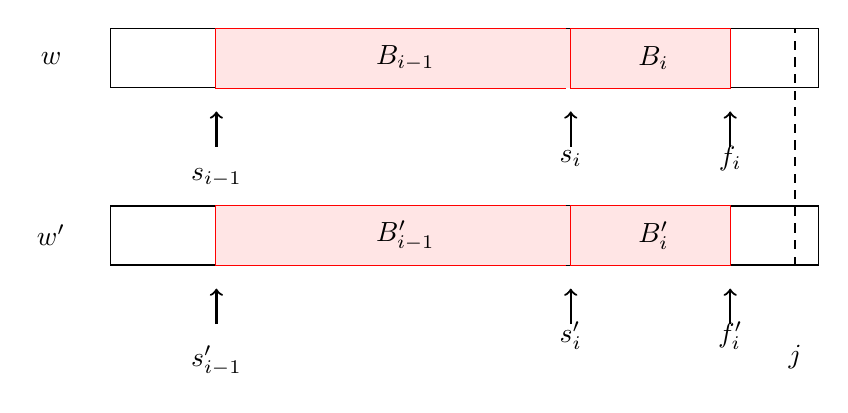
\begin{tikzpicture}[scale=1.5]
        % Main Rectangle w
        \draw (0,0) rectangle (6,0.5);
        \node at (-0.5, 0.25) {\(w\)};

        % Smaller Rectangle 1 - Border color red
        \draw[draw=red, thick] (0.9,0) rectangle (3.85,0.5);
        \draw[->, thick] (0.9,-0.5) -- (0.9,-0.2);
        \node[align=center, below] at (0.9,-0.6) {\(s_{i-1}\)};
        \fill[red!10] (0.9,0) rectangle (3.9,0.5);
        \node at (2.5,0.25) {$B_{i-1}$};

        % Smaller Rectangle 2 - Border color red
        \draw[draw=red, thick] (3.9,0) rectangle (5.25,0.5);
        \fill[red!10] (3.9,0) rectangle (5.25,0.5);
        
        \draw[->, thick] (3.9,-0.5) -- (3.9,-0.2);
        \draw[->, thick] (5.25,-0.5) -- (5.25,-0.2);
        \node at (3.9,-0.6) {$s_i$};
        \node at (5.25,-0.6) {$f_i$};

        % Label for Rectangle 3
        \node at (4.6,0.25) {$B_i$};

        % Dashed vertical line
        \draw[draw=black, thick, dashed] (5.8,-1.5) rectangle (5.8,0.5);
        \node[align=center, below] at (5.8,-2.1) {\( j\)};

        % Duplicate the structures for w' below
        % Offset for w' is -1.5 from w
        \begin{scope}[yshift=-1.5cm]
            \draw (0,0) rectangle (6,0.5);
            \node at (-0.5, 0.25) {\(w'\)};

            \draw[draw=red, thick] (0.9,0) rectangle (3.85,0.5);
            \draw[->, thick] (0.9,-0.5) -- (0.9,-0.2);
            \node[align=center, below] at (0.9,-0.6) {\(s'_{i-1}\)};
            \fill[red!10] (0.9,0) rectangle (3.9,0.5);
            \node at (2.5,0.25) {$B'_{i-1}$};

            \draw[draw=red, thick] (3.9,0) rectangle (5.25,0.5);
            \fill[red!10] (3.9,0) rectangle (5.25,0.5);
            
            \draw[->, thick] (3.9,-0.5) -- (3.9,-0.2);
            \draw[->, thick] (5.25,-0.5) -- (5.25,-0.2);
            \node at (3.9,-0.6) {$s'_i$};
            \node at (5.25,-0.6) {$f'_i$};

            \node at (4.6,0.25) {$B'_i$};
        \end{scope}
    \end{tikzpicture}
    \caption{Compression for $w$ and $w'$ which $f_i<j$.}
    \label{fig:case0}
\end{figure}

By Claim \ref{claim:c0}, we can conclude that there exists only one block $B_i'$ that can start inside $B_i$.


\label{case:b}    \item \emph{Case 1: \(s_i \leq j \leq f_i\)}. In this case, we observe the following claims:

    \begin{claim}\label{claim:c1si}
        If $s_i\leq j\leq f_i$, then $s_i=s_i'$.
    \end{claim}
    \begin{proof}[Proof of Claim \ref{claim:c1si}]
        We observe that $f_{i-1}<s_i\leq j$. Hence, by Claim \ref{claim:c0}, we have $B_k=B_k'$ for all $k\leq i-1$. This implies that $f_{i-1}=f'_{i-1}$. Hence, $s_i=f_{i-1}+1=f'_{i-1}+1=s_i'$.
    \end{proof}

    \begin{claim}\label{claim:c1fiprime}
        If $s_i\leq j\leq f_i$, then $f_i'\geq j$.
    \end{claim}
            \begin{figure}[ht!]
    \centering
    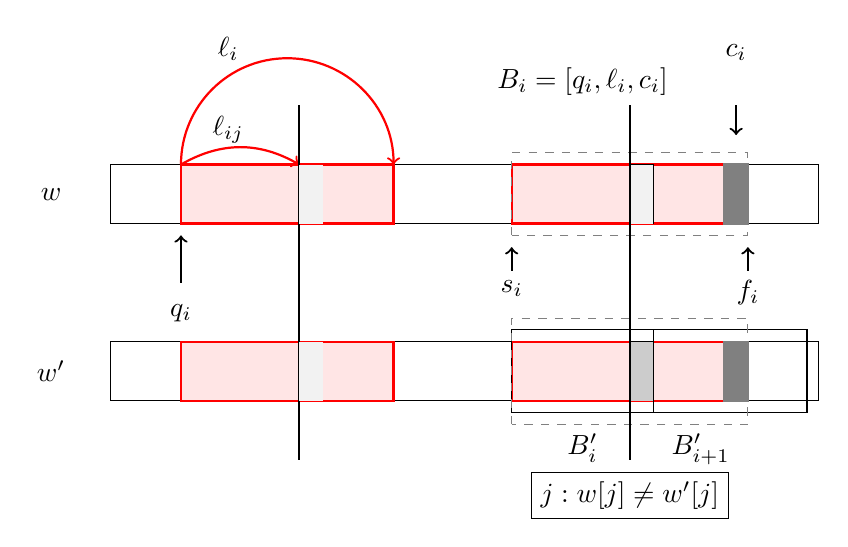
\begin{tikzpicture}[scale=1.5]
        % Main Rectangle w
        \draw (0,0) rectangle (6,0.5);
        \node at (-0.5, 0.25) {\(w\)};

        % Smaller Rectangle 1 - Border color red
        \draw[draw=red, thick, fill=red!10] (0.6,0) rectangle (2.4,0.5);
        \draw[->, thick] (0.6,-0.5) -- (0.6,-0.1);
        \node[align=center, below] at (0.6,-0.6) {\(q_i\)};

        % Semicircular arrow
        \draw[->, thick, red] (0.6,0.5) arc[start angle=180, end angle=0, radius=0.9cm];
        \path[->, thick, red] (0.6,0.5) edge[bend left] (1.6,0.5);
        
        \node[align=center, above] at (1.0,1.3) {\(\ell_i\)};
        \node[align=center, above] at (1.0,0.6) {\(\ell_{ij}\)};
        


        % Smaller Rectangle 2 - Border color red
        \draw[draw=red, thick, fill=red!10] (3.4,0) rectangle (5.2,0.5);
        
        \draw[->, thick] (5.3,1) -- (5.3,0.75);
        \node[align=center, below] at (5.3,1.6) {\(c_i\)};

        
        \node[align=center, above] at (4.0,1) {\(B_i=[q_i,\ell_i,c_i]\)};
        
        \draw[->, thick] (3.4,-0.4) -- (3.4,-0.2);
        \node[align=center, below] at (3.4,-0.4) {\(s_i\)};

        % CK indicator - Additional green block
        \draw[draw=gray, thick, fill=gray] (5.2,0) rectangle (5.4,0.5);
        
        

        \draw[->, thick] (5.4,-0.4) -- (5.4,-0.2);
        \node[align=center, below] at (5.4,-0.4) {\(f_i\)};
        

        % Main Rectangle w'
        \draw (0,-1.5) rectangle (6,-1);
        \node at (-0.5, -1.25) {\(w'\)};

        % Lower Smaller Rectangle 1 - Border color red
        \draw[draw=red, thick, fill=red!10] (0.6,-1.5) rectangle (2.4,-1);

        % Lower Smaller Rectangle 2 - Border color red
        \draw[draw=red, thick, fill=red!10] (3.4,-1.5) rectangle (5.2,-1);
        \draw (4.4,0) rectangle (4.6,0.5);

        
        
        \fill[gray!10] (4.4,0.0) rectangle (4.6,0.5);

        %Bi black block surrounding the all of it.
        
        \draw[draw=gray,dashed] (3.4,-0.1) rectangle (5.4,0.6);
        
        % \node[align=center, below] at (4.1,-0.3) {\( B_i\)};

        \draw (3.4,-1.6) rectangle (4.6,-0.9);
        \draw (4.4,-1.5) rectangle (4.6,-1);
        \fill[black!20] (4.4,-1.5) rectangle (4.6,-1);

        \draw (4.6,-1.6) rectangle (5.9,-0.9);
        
        \draw[draw=gray,dashed] (3.4,-1.7) rectangle (5.4,-0.8);
        
        
        \node[align=center, below] at (4.0,-1.7) {\( B'_i\)};
        \node[align=center, below] at (5.0,-1.7) {\( B'_{i+1}\)};
        
        
        % Lower Smaller Rectangle 3 - Border color green
        \draw[draw=gray, thick, fill=gray] (5.2,-1.5) rectangle (5.4,-1);
        
        %Line blue in the first block
        \draw[draw=black, thick] (1.6,-2) -- (1.6,1);
        \fill[gray!10] (1.6,0.0) rectangle (1.8,0.5);
        \fill[gray!10] (1.6,-1.5) rectangle (1.8,-1);
        


        % Line and index j
        \draw[draw=black, thick] (4.4,-2) -- (4.4,1);
        
        
        \node[draw=black,align=center, below] at (4.4,-2.1) {\( j:w[j] \neq w'[j]\)};
        

    \end{tikzpicture}
    \caption{Compressing \(w\) and \(w'\) when the character is located at $j$-position such as $s_i \leq s'_{k} \leq f_i$ and $s_i \leq s_{k+1} \leq f_i$.}
    \label{fig:case1_c_1}
\end{figure}
    \begin{proof}[Proof of Claim \ref{claim:c1fiprime}]
        Suppose for contradiction that $f_i'<j$. We first observe that $w'[s_i',f_i'-1]$ is the longest substring of $w'[1,s_i'-1]$ that starts at $s_i'$. Next, we observe that $w[s_i,j-1]$ is a substring of $w[1,s_i-1]$. Note that, since $j$ is the only index where $w$ and $w'$ differ, we further observe that 
        \begin{equation}\label{eq1}
            w[s_i,j-1]=w'[s_i,j-1]=w'[s_i',j-1],
        \end{equation}
        where the last equality comes from Claim \ref{claim:c1si}. Similarly, since $s_i\leq j$, we have 
        \begin{equation}\label{eq2}
            w[1,s_i-1]=w'[1,s_i-1]=w'[1,s_i'-1].
        \end{equation}
        By Equation \eqref{eq1} and Equation \eqref{eq2}, along with the fact that $w[s_i,j-1]$ is a substring of $w[1,s_i-1]$ that we observed before, we have that $w'[s_i',j-1]$ is a substring of $w'[1,s_i'-1]$. Contradiction because $w'[s_i',j-1]$ is a \emph{longer} substring of $w'[1,s_i'-1]$ than $w'[s_i',f_i'-1]$ starting at $s_i'$! Hence, the LZ77 algorithm would have picked $w'[s_i',j-1]$ instead of $w'[s_i',f_i'-1]$ when constructing $B_i'$. This contradiction is due to the assumption that $f_i'<j$. Hence, we can conclude that $f_i'\geq j$.
        \end{proof}


    
\begin{claim}\label{claim:c1fprime+1geqfi}
    If $s_i\leq j\leq f_i$, then $f_{i+1}'\geq f_i$.
    \end{claim}
        % In Figure \ref{fig:case_1_c_2}, we observe blocks of $w'$ start inside blocks of $w$.

    \begin{figure}[ht!]  % 'htbp' suggests placement options
    \centering
    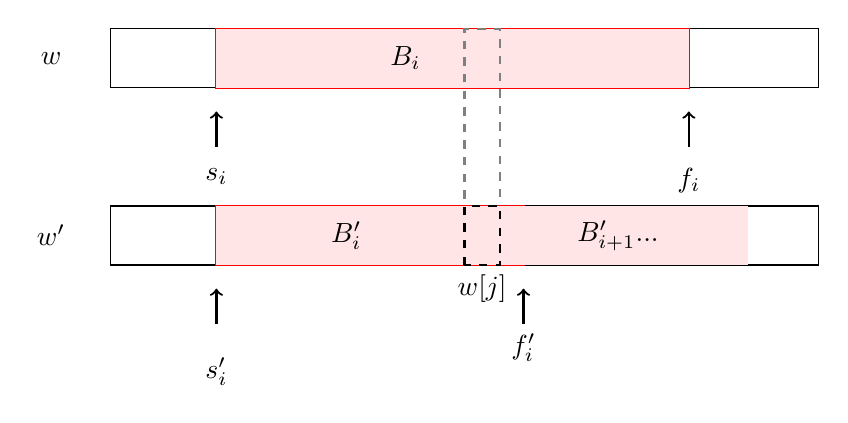
\begin{tikzpicture}[scale=1.5]
        % Main Rectangle w
        \draw (0,0) rectangle (6,0.5);
        \node at (-0.5, 0.25) {\(w\)};

        % Smaller Rectangle 1 - Border color red
        \draw[draw=red, thick] (0.9,0) rectangle (4.9,0.5);
        
        \draw[->, thick] (0.9,-0.5) -- (0.9,-0.2);
        \node[align=center, below] at (0.9,-0.6) {\(s_i\)};
        \draw[->, thick] (4.9,-0.5) -- (4.9,-0.2);
        \node[align=center, below] at (4.9,-0.6) {\(f_i\)};
        \fill[red!10] (0.9,0) rectangle (4.9,0.5);
        \node at (2.5,0.25) {$B_{i}$};


        % Dashed vertical line
        \draw[draw=gray, thick, dashed] (3.0,-1.5) rectangle (3.3,0.5);
        \node[align=center, below] at (3.15,-1.5) {\( w[j]\)};

        % Duplicate the structures for w' below
        % Offset for w' is -1.5 from w
        \begin{scope}[yshift=-1.5cm]
            \draw (0,0) rectangle (6,0.5);
            \node at (-0.5, 0.25) {\(w'\)};

            \draw[draw=red, thick] (0.9,0) rectangle (3.5,0.5);
            
            \draw[->, thick] (0.9,-0.5) -- (0.9,-0.2);
            \node[align=center, below] at (0.9,-0.7) {\(s'_i\)};
            \fill[red!10] (0.9,0) rectangle (3.5,0.5);
            \node at (2.0,0.25) {$B'_{i}$};
            
            \draw[->, thick] (3.5,-0.5) -- (3.5,-0.2);
            
            \node at (3.5,-0.7) {$f'_i$};

            % \draw[draw=red, thick] (3.5,0) rectangle (4.9,0.5);
            \fill[red!10] (3.5,0) rectangle (5.4,0.5);
            \node at (4.3,0.25) {$B'_{i+1}...$};
            
            \draw[draw=black, thick, dashed] (3.0,-0.0) rectangle (3.3,0.5);
        \end{scope}
    \end{tikzpicture}
    \caption{Compression for $w$ and $w'$ which $f'_{i+1}\geq j$.}
    \label{fig:case_1_c_2}
\end{figure}
    
\begin{proof}[Proof of Claim \ref{claim:c1fprime+1geqfi}]
    Suppose for contradiction that $f_{i+1}' < f_i$.  Observe that if $f_{i+1}' < f_i$ then we have $f_i' < s_{i+1}' < f_{i+1}' < f_i$. By definition of LZ77-Block-Based we observe that $w'[s_{i+1}',f_{i+1}'-1]$ was the longest possible substring of $w'[1,f_i']$ starting at $s_{i+1}'$. Next, we observe that $w[j+1,f_i-1]$ is a substring of $w[1, f_{i-1}]$. since $f_{i-1}<j$ we further observe that:
    \begin{equation}
    w[1, f_{i-1}]=w'[1, f_{i-1}]  ,    
    \label{eq:case1_b_eq1}
    \end{equation}
    and
    \begin{equation}
   w[j+1,f_i-1]=w'[j+1,f_i-1].
   \label{eq:case1_b_eq2}
    \end{equation}
By Equation \eqref{eq:case1_b_eq1} and Equation \eqref{eq:case1_b_eq2}, along with the fact that \( w[s_i, j-1] \) is a substring of \( w[1, s_i - 1] \) that we observed before, we note that \( w'[s_{i+1}', f_i - 1] \) is a substring of \( w'[1, f_{i-1}] \). However, since $f_{i-1} = f_{i-1}' < f_i'$ it follows that \( w'[s_{i+1}', f_i - 1] \) is also a substring of \( w'[1, f_i'] \). This is a contradiction as \( w'[s_{i+1}', f_i - 1] \) is longer than \( w'[s_{i+1}', f_{i+1}' - 1] \) which means that LZ77-Block-Based would have selected the longer block. Thus, \( f_{i+1}' \geq f_i \). 
\end{proof}
     
Taken together, by Claim \ref{claim:c1si}, Claim \ref{claim:c1fiprime}, and Claim \ref{claim:c1fprime+1geqfi}, we have $s_i'=s_i$ and $s_{i+2}'=f_{i+1}'+1\geq f_i +1 > f_i$. This implies that at most two blocks $B_i'$ and $B_{i+1}'$ can start inside $B_i$. In particular, for block $B_{i+2}'$ we have $s_{i+2}' > f_{i+1}' \geq f_i$. This completes the proof of Case 1.

\label{case:c} \item \emph{Case 2: $j<s_i$.} If $f'_{k}\geq f_i $ then block $B_{k+1}'$ does not start inside block $B_i$ as $s_{k+1}' > f_{k}' \geq f_i$ so that block $B_i$ trivially contains at most 1 block. Thus, we may assume without loss of generality that $f'_k<f_i$. 

Since the block $B_k'$ starts inside $B_i$ it is useful to define the offset $z \coloneqq s'_k-s_i$. In the figure \ref{fig:case_2_a} can be shown:

%%%%%%%%
        \begin{figure}[ht!]  
    \centering
    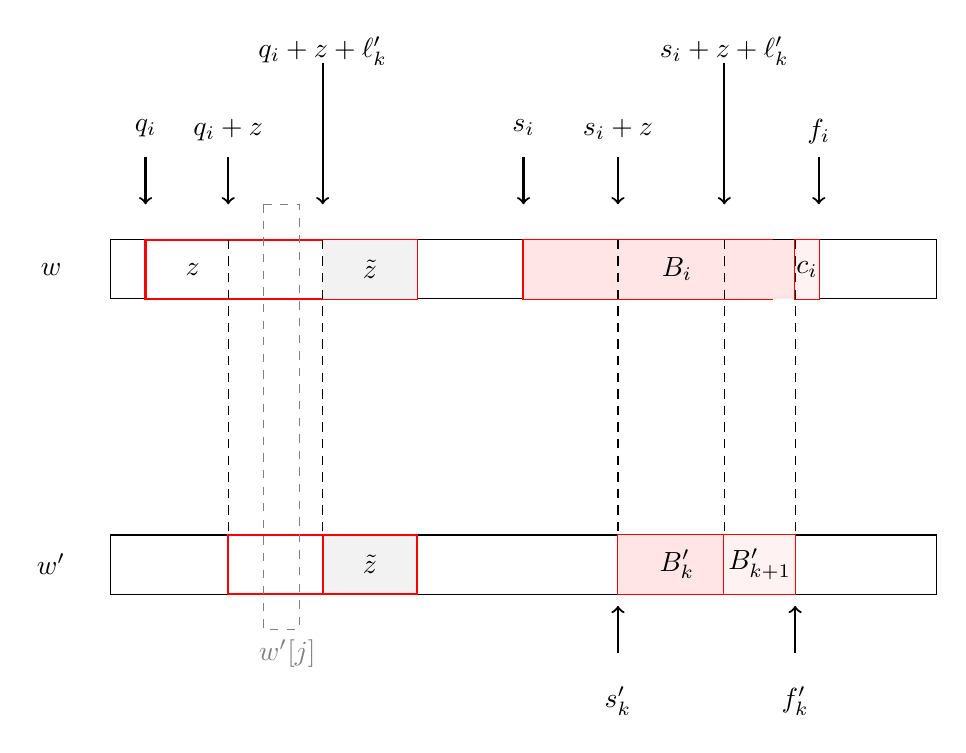
\begin{tikzpicture}[scale=1.5]
        % Main Rectangle w
        \draw (0,0) rectangle (7,0.5);
        \node at (-0.5, 0.25) {\(w\)};
        
        % Smaller Rectangle 2 - Border color red
        \draw[draw=red, thick] (0.3,0) rectangle (2.6,0.5);
        % Smaller Rectangle 2 - Border color red
        \draw[draw=red, thick] (3.5,0) rectangle (5.6,0.5);
        \fill[red!10] (3.5,0) rectangle (5.8,0.5);
        \draw[draw=red, thick] (5.8,0) rectangle (6.0,0.5);
        \fill[red!5] (5.8,0) rectangle (6.0,0.5);
        \node at (5.9,0.25) {$c_{i}$};
        

        \draw[->, thick] (3.5,1.2) -- (3.5,0.8);
        \node[align=center, below] at (3.5,1.6) {\(s_i\)};
        \draw[->, thick] (4.3,1.2) -- (4.3,0.8);
        \node[align=center, below] at (4.3,1.6) {\(s_{i}+z\)};
        
        
        
        
        \draw[->, thick] (6.0,1.2) -- (6.0,0.8);
        \node[align=center, below] at (6.0,1.6) {\(f_i\)};

        \node at (4.8,0.25) {$B_{i}$};

    % w'
    \draw (0,-2) rectangle (7,-2.5);
    \fill[gray!10] (1.8,-2) rectangle (2.6,-2.5);
    \fill[gray!10] (1.8,0) rectangle (2.6,0.5);

    \node at (0.7,0.25) {$z$};
    \node at (2.2,0.25) {$\tilde{z}$};
    \node at (2.2,-2.25) {$\tilde{z}$};
    
    
    \node at (-0.5, -2.25) {\(w'\)};
    \draw[draw=red, thick] (1.0,-2) rectangle (1.8,-2.5);
    \draw[dashed] (1.0,0.5) rectangle (1.0,-2.0);
    \draw[dashed] (1.8,0.5) rectangle (1.8,-2.0);
    \draw[dashed,draw=gray] (1.3,0.8) rectangle (1.6,-2.8);
    \node[color=gray] at (1.5,-3.0) {$w'[j]$};
    
    
    \draw[draw=red, thick] (1.8,-2) rectangle (2.6,-2.5);
    \draw[draw=red, thick] (4.3,-2) rectangle (5.8,-2.5);
    \node[align=center, below] at (0.3,1.6) {\(q_i\)};
    \draw[->, thick] (0.3,1.2) -- (0.3,0.8);

    \node[align=center, below] at (1.0,1.6) {\(q_i+z\)};
    \draw[->, thick] (1.0,1.2) -- (1.0,0.8);

    \node[align=center, below] at (1.8,2.3) {\(q_i+z+\ell'_k\)};
    \draw[->, thick] (1.8,2.0) -- (1.8,0.8);
    
    \fill[red!10] (4.3,-2) rectangle (5.8,-2.5);
    
    \draw[draw=red, thick] (5.2,-2) rectangle (5.2,-2.5);
    \fill[red!5] (5.2,-2) rectangle (5.8,-2.5);
    
    
    \draw[->, thick] (4.3,-3.0) -- (4.3,-2.6);
    \node[align=center, below] at (4.3,-3.2) {\(s'_{k}\)};
    
    
    \draw[->, thick] (5.8,-3.0) -- (5.8,-2.6);
    \node[align=center, below] at (5.8,-3.2) {\(f'_{k}\)};
    
    \node at (4.8,-2.25) {$B'_{k}$};
    \node at (5.5,-2.25) {$B'_{k+1}$};


    \draw[dashed] (4.3,0.5) rectangle (4.3,-2.0);
    \draw[dashed] (5.2,0.5) rectangle (5.2,-2);
    \draw[dashed] (5.8,0.5) rectangle (5.8,-2.);
    
    
    \node[align=center, below] at (5.2,2.3) {\(s_{i}+z+\ell'_k\)};
    \draw[->, thick] (5.2,2.0) -- (5.2,0.8);
    
        
        

        
    \end{tikzpicture}
    \caption{Compression for $w$ and $w'$ which $j<s_i$}
    \label{fig:case_2_a}
\end{figure}

         
        
%%%%%%%%

    
We observe the following claims:
    \begin{claim}
    \label{claim:case2:a}
    If $j<s_i$ then $j \leq q_i+z+\ell'_k$.
    \end{claim}

\begin{proof}[Proof of Claim \ref{claim:case2:a}]
    Suppose for contradiction that $j>q_i+z+\ell_k'$, then we note $w'[s'_k,f'_k-1] $ is the longest possible substring of $w'[1,s'_{k}-1]$ that starts at $s'_k$. Next we observe that $w[q_{i}+z,q_i+z+\ell_k']$ is trivially a substring of $w[1,j-1]$ since we assumed $j>q_i+z+\ell_k'$. Furthermore, we have $w[q_{i}+z,q_i+z+\ell_k']=w[s_{i}+z,s_i+z+\ell_k']$ since $s_i+z+\ell_k'=f_k'<f_i$. Therefore,        
        $w[s_{i}+z,s_i+z+\ell_k']$ is a substring of $w[1,j-1]$. We further observe that

        \begin{equation}
           w[s_i+z,s_i+z+\ell_k']=w[s_k',f_k']=w'[s_k',f_k']
           \label{equation:case2:a:1}
        \end{equation}
    
    and
    \begin{equation}
        w[1,j-1]=w'[1,j-1].
        \label{equation:case2:a:2}
    \end{equation}


By equation \eqref{equation:case2:a:1} and \eqref{equation:case2:a:2} we have that $w'[s'_k,f_k']$ is a substring of $w'[1,j-1]$, which is a substring of $w'[1,s_k'-1]$. %We should remind the fact that \textcolor{blue}{$w[s_i+z,j-1]$} is a substring of \textcolor{red}{$w[1,s_i+z-1]$} that we observed before,
Contradiction because $w'[s'_k,f_k']$ is a \emph{longer} substring of $w'[1,s'_{k'}-1]$ than $w'[s'_k,f'_k-1]$ starting at $s'_k$! Hence, the LZ77 algorithm would have picked $w'[s'_k,f_k']$ instead of $w'[s'_k,f'_k-1]$. This contradiction is due to the assumption that $j>q_i+z+\ell_k$. Hence, we can conclude that $j\leq q_i+z+\ell_k$.
\end{proof}

    



    \begin{claim}
    \label{claim:case2:b}
    If $j<s_i$ then $f'_{k+1}\geq f_i$.
    \end{claim}
    \begin{proof}[Proof of Claim 
    \ref{claim:case2:b}]


Suppose for contradiction that \( f'_{k + 1} < f_i \). 
By the definition of the LZ77-Block-Based compression algorithm, we first observe that $w'[s_{k+1}',f_{k+1}'-1]$ is the longest possible substring of $w'[1,s_{k+1}'-1]$ starting at $s_{k+1}'$. 
It is useful for our proof to define $\tilde{z} \coloneqq (f_i-1)-f_k'$. We observe that, by the definition of the LZ77-Block-Based compression algorithm, 
\begin{equation}\label{eqqisi}
    w[q_i + z + \ell'_k + 1, q_i + z + \ell'_k + \tilde{z}] = w[s_i + z + \ell'_k + 1, s_i + z + \ell'_k + \tilde{z}],    
\end{equation}
since the LHS of \eqref{eqqisi} is copied to the RHS of \eqref{eqqisi} when we run the algorithm. We also observe that
\begin{align}\label{eq:case2:11}
    s_i + z + \ell'_k + 1 &= s_i + (s_k'-s_i) + \ell'_k + 1 \nonumber\\
    &= s_k' + \ell_k' + 1 \nonumber \\
    &= f_k'+1 \nonumber \\
    &= s_{k+1}',
\end{align}
and
\begin{align}\label{eq:case2:22}
    s_i + z + \ell'_k + \tilde{z} &= s_i + (s_k'-s_i) + \ell'_k + (f_i-1)-f_k' \nonumber\\
    &= s_k' + \ell'_k + (f_i-1) - f_k'\nonumber \\
    &= f_k' + (f_i-1) - f_k' \nonumber\\
    &= f_i - 1.
\end{align}
Together with Equation \eqref{eq:case2:11} and \eqref{eq:case2:22}, by Equation \eqref{eqqisi} we have
\begin{equation}\label{c}
    w[q_i + z + \ell'_k + 1, q_i + z + \ell'_k + \tilde{z}] = w[s_{k+1}', f_i-1].
\end{equation}


    % \begin{equation}
    % \label{eq:case2:b:1}
    %     w[q_i + z + \ell'_k + 1, q_i + z + \ell'_k + \tilde{z}] = w[s_i + z + \ell'_k + 1, f_i-1]
    % \end{equation}

Due to Claim \ref{claim:case2:a}, we have $j<q_i+z+\ell'_k+1$. Since $j$ was the unique index where $w[j]\neq w'[j]$, we have
\begin{equation}\label{a}
    w[q_i + z + \ell'_k + 1, q_i + z + \ell'_k + \tilde{z}] = w'[q_i + z + \ell'_k + 1, q_i + z + \ell'_k + \tilde{z}],
\end{equation}
and
\begin{equation}\label{b}
    w[s_{k+1}', f_i-1] = w'[s_{k+1}', f_i-1].
\end{equation}
Applying Equations \eqref{a} and \eqref{b} to Equation \eqref{c}, we obtain
\begin{equation}
    w'[q_i + z + \ell'_k + 1, q_i + z + \ell'_k + \tilde{z}] = w'[s_{k+1}', f_i-1].
\end{equation}
Since $w'[q_i + z + \ell'_k + 1, q_i + z + \ell'_k + \tilde{z}]$ is a substring of $w'[1,s_{k+1}'-1]$, we observe that $w'[s_{k+1}', f_i-1]$ is a substring of $w'[1,s_{k+1}'-1]$ starting at $s_{k+1}'$. Contradiction since $f_i-1 > f_{k+1}'-1$, which implies the LZ77-Block-Based compression algorithm would have picked $w'[s_{k+1}', f_i-1]$ instead of $w'[s_{k+1}', f_{k+1}'-1]$ when constructing the block $B_{k+1}'$. This contradiction is due to the assumption $f_{k+1}'<f_i$. Hence, we can conclude that $f_{k+1}'\geq f_i$.

Taken together, by Claim \ref{claim:case2:a} and Claim \ref{claim:case2:b}, we have $j\leq q_i+z+\ell'_k$ and $f'_{k+1}\geq f_i$. this implies that at most two blocks $B'_k$ and $B'_{k+1}$ can start inside $B_i$. In particular, for block $B'_{k+2}$ we have $s'_{k+2}\geq f'_{k+1}\geq f_i$. This completes the proof of Case 2.
\end{proof}

% Finalize the proof for Case 2)

\end{enumerate}

% (Finalize the proof, combining all the three cases)
We have considered \lemref{lemma:start_inside}, where in Case 0 we showed that if $f_i<j$, then $B_k=B_k'\,\,\forall k\leq i$ what means, in fact, for Claim \ref{claim:c0}  there is only a block $B'_i$ that start inside.
In Case 1 we showed in Claim \ref{claim:c1si} that If $s_i\leq j\leq f_i$, then $s_i=s_i'$, that explains when both start position are the same, so then there is only one block that can start inside $B_i$. However, we showed in Claim \ref{claim:c1fiprime} that if $s_i\leq j\leq f_i$, then $f_i'\geq j$ what means there are two blocks $B'_i$ and $B'_{i+1}$ that start inside $B_i$. Eventually, by Claim \ref{claim:c1fprime+1geqfi} if $s_i\leq j\leq f_i$, then $f_{i+1}'\geq f_i$ and this condition implies immediately since $s_i=s'_i$ that at most two blocks $B'_i$ and $B'_{i+1}$ can start inside $B_i$.
In Case 2, we proved in Claim \ref{claim:case2:a} that if $j<s_i$ then $j \leq q_i+z+\ell'_k$ and in Claim \ref{claim:case2:b} if $j<s_i$ then $f'_{k+1}\geq f_i$. We established that taking all possible assumptions of our lemma are valid. By proving that \emph{at most two blocks can start inside $B_i$} holds in all scenarios, we have proved that the lemma is true in general.
Therefore, we conclude that \lemref{lemma:start_inside} is proven.
\end{proof}



\newcommand{\claimGSstatement}{
Let $\compress:(\Sigma)^*\rightarrow(\Sigma')^*$ be the LZ77 compression function  and $w,w'$ be strings of length $n$ and $w\sim w'$. Then
    $\left| \left| \compress(w) \right| - \left| \compress(w') \right| \right| \leq  t_2(2\left\lceil \log n \right \rceil + \left\lceil \log |\Sigma|\right \rceil).$
}
\begin{claim}\claimlab{claim:compress:GS}
\claimGSstatement
\end{claim}

\begin{proof}[Proof of {\claimref{claim:compress:GS}}]
Let $(B_1,\ldots,B_t)\gets\compress(w)$ and $(B_1',\ldots,B_{t'}')\gets\compress(w')$. 
We first observe that there are $t$ blocks in $\compress(w)$ and encoding each block we need $2 \lceil\log n\rceil + \lceil\log|\Sigma|\rceil$ bits, since each block consists of two integers $q_i$ and $\ell_i$, and one character $c_i$ with $0\leq q_i,\ell_i\leq n-1$ and $c_i\in\Sigma$. Hence, $|\compress(w)| = t(2\lceil\log n\rceil + \lceil\log|\Sigma|\rceil).$ and 
$|\compress(w')| = t'(2\lceil\log n\rceil + \lceil\log|\Sigma|\rceil).$
Then,     $\left| \compress(w) \right| - \left| \compress(w') \right| =\left|t-t'\right||2\lceil\log n\rceil + \lceil\log|\Sigma|\rceil|.$ By \claimref{claim:set:blocksm2:GS} above, we observe that $|t-t'|\leq t_2$. Hence, we have $\left|\left| \compress(w) \right| - \left| \compress(w') \right|\right|\leq t_2(2\lceil\log n\rceil + \lceil\log|\Sigma|\rceil).$
\end{proof}

\subsection{Counting Type-2 Blocks}\applab{app:missingproofC}

\begin{remindertheorem}{\lemref{lemma:length_cases_total}}
    \lemblocknumstatement
\end{remindertheorem}

\begin{proof}
We consider the following claims:
\begin{claim}
\claimlab{claim:length_cases_total_a}


    If $i\in\B_2$ then either (1) $s_i\leq j\leq f_i$ or (2) $j-\ell_i < q_i \leq j$.
\end{claim}
\begin{proof}[Proof of \claimref{claim:length_cases_total_a}]
    We first observe that it has to be either $j\geq s_i$ or $j<s_i$.
    \begin{itemize}
        \item If $j\geq s_i$, then we want to show that $s_i\leq j\leq f_i$. Suppose for contradiction that $j>f_i$. Then we have $w[1,f_i]=w'[1,f_i]$, i.e., two substrings are identical. Hence, by definition of the LZ77 compression algorithm, the block constructions are also the same, i.e., $s_i=s_i'$ and $f_i=f_i'$, where $s_i'$ and $f_i'$ denote the starting and finishing index for the block $B_i'$ for compressing $w'$. This implies that $\M_i=\{i\}$ and $i\in\B_1$. Contradiction since $i\in\B_2$. Hence, we have $s_i\leq j\leq f_i$ if $j\geq s_i$.
        \item If $j<s_i$, then we want to show that $j-\ell_i<q_i\leq j$, i.e., $q_i\leq j < q_i+\ell_i$. 
        
        
        Suppose for contradiction that $j\not\in[q_i,q_i+\ell_i-1]$. Then we have 
        \begin{equation}\label{eq:C9C2}
            w[s_i,f_i-1]=w[q_i,q_i+\ell_i-1]=w'[q_i,q_i+\ell_i-1]=w'[s_i,f_i-1].
        \end{equation}
        Let $k$ be the smallest element in $\M_i$, i.e., $s_i\leq s_k'\leq f_i$ but $s_{k-1}'<s_i$. 
        \begin{itemize}
            \item If $s_k'=f_i$, then if there is another $k'\in\M_i$ with $k'\neq k$, then by choice of $k$, we have $k<k'$ and therefore $s_{k'}'>f_k'>s_k'=f_i$. Hence, $|\M_i|= 1$ and $i\in\B_1$. Contradiction!
            \item If $s_i\leq s_k'\leq f_i-1$, then from Equation \eqref{eq:C9C2} and from the fact that $f_i=s_i+\ell_i$, we observe that the substring $w'[s_i,f_i-1]$ can be obtained by shifting the substring $w'[q_i,q_i+\ell_i-1]$ by $s_i-q_i$. Hence,
            \begin{align*}
                w'[s_k',f_i-1] &= w'[s_k',s_i+\ell_i-1]\\
                &=w'[s_k'-(s_i-q_i),s_i+\ell_i-1-(s_i-q_i)]\\
                &=w'[q_i+(s_k'-s_i),q_i+\ell_i-1],
            \end{align*}
            which implies that $f_k'\geq f_i$ by definition of the LZ77 compression algorithm. If there is another $k'\in\M_i$ with $k'\neq k$, then by choice of $k$, we have $k<k'$ and therefore $s_{k'}'>f_k'\geq f_i$. Hence, $|\M_i|=1$ and $i\in\B_1$. Contradiction!
        \end{itemize}
        Hence, we have $j\in[q_i,q_i+\ell_i-1]$ and therefore $q_i\leq j<q_i+\ell_i$ if $j<s_i$.
    \end{itemize}
    Taken together, we can conclude that if $i\in\B_2$ then either $s_i\leq j\leq f_i$ or $q_i\leq j<q_i+\ell_i$ must hold.
\end{proof}

\begin{claim}
\claimlab{claim:length_cases_total_b}
    If $i_1,i_2\in\B_2$ then $(q_{i_1},\ell_{i_1})\neq(q_{i_2},\ell_{i_2})$. 
\end{claim}
\begin{proof}[Proof of \claimref{claim:length_cases_total_b}]
    Suppose for contradiction that $\exists i_1,i_2 \in \mathcal{B}_2 $ such that $(q_{i_1},\ell_{i_1})=(q_{i_2},\ell_{i_2})$. Without loss of generality, assume $i_1<i_2$. Now, we consider the following cases:
\begin{enumerate}
\label{case:length_cases_total:case:a} \item \emph{Case 1: $j<s_{i_1}$}. 
Since $i_1<i_2$ we then have $j<s_{i_1}<s_{i_2}$. Let $B_{i_1}=[q_{i_1},\ell_{i_1},c_{i_1}]$ and $B_{i_2}=[q_{i_2},\ell_{i_2},c_{i_2}]$ be  the blocks $B_{i_1}$ and $B_{i_2}$ of the LZ77 compression function $\compress:(\Sigma)^*\rightarrow(\Sigma')^*$ (Resp. w'). Let $k \in \S_{i_2}$ be the smallest element in  $\S_{i_2}$. Since $q_{i_1}=q_{i_2}$ and $\ell_{i_1}=\ell_{i_2}$, we first observe that, 

\[w[q_{i_1},q_{i_1}+\ell_{i_1}-1]=w[s_{i_1},f_{i_1}-1]=w'[s_{i_1},f_{i_1}-1],\]
and
\[w[q_{i_2},q_{i_2}+\ell_{i_2}-1]=w[s_{i_2},f_{i_2}-1]=w'[s_{i_2},f_{i_2}-1],\]

Therefore, we have that,
\[w'[s'_{k},f_{i_2}-1]=w'[s_{i_1}+(s'_{k}-s_{i_2}),f_{i_1}-1].\]

By definition of LZ77 we know that, $f'_k\geq f_{i_2}.$ Now, suppose for contradiction that $f'_k<f_{i_2}$, then $w'[s'_k,f'_{k}-1]$ is the longest substring of $w'$ starting at $s'_k$, but, $w'[s'_k,f_{i_2}-1]=w'[s_{i_1}+(s'_k-s_{i_2}),f_{i_1}-1]$
implies that $w'[s'_k,f_{i_2}-1]$ is a substring of $w'$ but $f_{i_2}-1>f'_k-1$ that is a contradiction!. Then $f'_k \geq f_{i_2}$.
    


%Now, to prove this, lets suppose for contradiction that $f'_k<f_{i_2}$. We first observe that: $w'[s'_{k},f'_{k}-1]$ is the longest substring of $w'$\sebastian{Correct this $1,s_k-1$} starting at $s'_k-1$ but, \[w'[s'_k,f_{i_2}-1]=w'[s_{i_1}+(s'_k-s_{i_2},f_{i_1}-1)].\] This implies that $w'[s'_k,f_{i_2}-1]$ is a subtring of $w'$ but $f_{i_2}-1> f'_{k}-1$. This is a contradiction!. Therefore $f'_k\geq f_{i_2}.$ 

Finally, if there is another $k' \in \S_{i_2}$ such that $k' \neq k$ then, by choice of $k$, we have $k<k'$ and therefore $s_{k'}' > f_k' \geq f_{i_2}$. This contradicts the definition of $\S_{i_2}$ since block $B_k'$ does not start inside block $B_{i_2}$. It follows that $\left| \S_{i_2}\right| \leq 1$ and therefore $i_2\in\B_1$. This is a contradiction!. Hence, we can conclude that if $i_1,i_2\in\B_2$ then $(q_{i_1},\ell_{i_1})\neq(q_{i_2},\ell_{i_2})$.

\label{case:length_cases_total:case:b}  \item \emph{Case 2: $j \geq s_{i_1}$}.
We then observe $s_{i_1} \leq j<f_{i_1}$ (if $f_{i_1}\leq j$ then only one block would have started inside $B_{i_1}$ by observing $w[s_{i_1},f_{i_1}-1]=w'[s_{i_1},f_{i_1}-1]$, hence $i\in \B_1$, which is a contradiction since $i\in\B_2$). And since we assumed $i_1<i_2$, we further have $s_{i_1} \leq j<f_{i_1}<s_{i_2}$. Let $B_{i_1}=[q_{i_1},\ell_{i_1},c_{i_1}]$ and $B_{i_2}=[q_{i_2},\ell_{i_2},c_{i_2}]$ be  the blocks $B_{i_1}$ and $B_{i_2}$ of the LZ77 compression function $\compress:(\Sigma)^*\rightarrow(\Sigma')^*$. Let $k' \in \S_{i_2}$ be the smallest element in  $\S_{i_2}$, moreover, since the block $B'_{k'}$ starts inside $B_{i_2}$ it is useful to define that $\ell_{i_2}=f_{i_2}-1-s'_k$, so that, $s'_k=f_{i_2}-1-\ell_{i_2}$. We also know that $q_{i_1}=q_{i_2}$ and $\ell_{i_1}=\ell_{i_2}$, so we observe for $q_1$ that, 
\[w[q_{i_1},q_{i_1}+\ell_{i_1}-1]=w[s_{i_2},f_{i_2}-1]=w'[s_{i_2},f_{i_2}-1]\]

and for $q_2$ since $q_1=q_2$, we have that: 
\[w[q_{i_1},q_{i_1}+\ell_{i_1}-1]=w'[q_{i_2},q_{i_2}+\ell_{i_2}-1]=w[s_{i_1},f_{i_1}-1]\]
Furthermore, by the equalities we can see that:

\begin{equation}
  % w'[s'_{k},f_{i_2}-1-s'_k+1]=w'[q_{i_1}+(s'_{k}-s_{i_2}),q_{i_1}+\ell_{i_1}-1-(q_{i_1}+(s'_{k}-s_{i_2})].  
  w'[q_{i_2},q_{i_2}+\ell_{i_2}-1] = w'[s_{i_2},f_{i_2}-1],
  \label{claim10:case2}
\end{equation}
This intuitevely means that, any two substrings ending at the index $q_{i_2}+\ell_{i_2}-1$ and $f_{i_2}-1$, respectively, with the same length, are exactly the same. 

On the other hand, we know that:
\begin{align}
  % f_{i_2}-1-s'_{k}+1=f_{i_2}-s'_{k}  
  (f_{i_2}-1)-s'_k = (q_{i_2}+\ell_{i_2}-1-q_{i_2}+(s'_k-s_{i_2})).
  \label{claim10:case2:fact}
\end{align}

Taken RHS of \eqref{claim10:case2:fact} we have that:
\begin{align}
   % q_{i_1}+\ell_{i_1}-1-(q_{i_1}+(s'_{k}-s_{i_2}))&= -s'_k+s_{i_2}+\ell_{i_1} \nonumber \\
   % &= f_{i_2}-s'_k 
   (q_{i_2}+\ell_{i_2}-1-q_{i_2}+(s'_k-s_{i_2}))&=\ell_{i_2}-1-s'_k+s_{i_2}\nonumber \\
   &= s_{i_2}+\ell_{i_2}-1-s'_k\nonumber \\
   &=f_{i_2}-1-s'_k
   \label{claim10:case2:RHS}
\end{align}

So then, because of \eqref{claim10:case2:RHS} the RHS is the same as LHS, then we can say that:
\begin{equation}
w'[s'_k, f_{i_2} - 1] = w'[q_{i_2} + (s'_k - s_{i_2}), q_{i_2} + \ell_{i_2} - 1]
\end{equation}

% \begin{equation}
%   % w'[s'_{k},f_{i_2}-s'_k]=w'[q_{i_1}+(s'_{k}-s_{i_2}),f_{i_2}-s'_k].
  

% \end{equation}

By definition of LZ77, we know by a similar reason of case 1 that $f_k' \geq f_{i_2}$. If there is another $k'' \in \S_{i_2}$ such that $k'' \neq k'$ then, by choice of $k'$ we have $k'<k''$, $s_{k''} > f_k' \geq f_{i_2}$. This contradicts the definition of $\S_{i_2}$ since block $B_{k''}$ does not start inside block $B_{i_2}$. It follows that $\left| \S_{i_2}\right| \leq 1$ and therefore $i_2\in\B_1$. This is a contradiction!

%Therefore $w'[s'_k,f_{i_2}-1]=w'[s_{i_2},f_{i_2}-1]$. We know by conclusion of Claim \ref{claim:length_cases_total_a} that if $s_{i_1} \leq j \leq f_{i_1}$ then $f'_{k+1}\geq f_{i_1}$, it means that $i\in \B_{1}$. Contradiction!. Hence, we can conclude that if $i_1,i_2\in\B_2$ then $(q_{i_1},\ell_{i_1})\neq(q_{i_2},\ell_{i_2})$.
\end{enumerate}
Hence, we can conclude that if $i_1,i_2\in\B_2$ then $(q_{i_1},\ell_{i_1})\neq(q_{i_2},\ell_{i_2})$.   
\end{proof}


\begin{claim}
\claimlab{claim:length_cases_total_c}
    Let $\B_2^\ell\coloneqq\{i\in\B_2:\ell_i=\ell\}$ and suppose that $s_{i^*}\leq j\leq f_{i^*}$ for some $i^*\in[t]$. Then $|\B_2^\ell|\leq\ell$ for all $\ell\neq \ell_{i^*}$, and $|\B_2^{\ell_{i^*}}|\leq\ell_{i^*}+1$.
\end{claim}

\begin{proof}[Proof of \claimref{claim:length_cases_total_c}]
We first observe from \claimref{claim:length_cases_total_a} that if $i\in\B_2$, either $s_i\leq j\leq f_i$ or $j-\ell_i<q_i\leq j$ holds. Let $i^*\in[t]$ be the unique index such that $s_{i^*}\leq j\leq f_{i^*}$.
\begin{itemize}
    \item If $\ell\neq\ell_{i^*}$, then for all $i\in\B_2^\ell$, we have $j-\ell_i<q_i\leq j$ since $j\not\in[s_i,f_i]$ for all $i\in\B_2^\ell$. Suppose for contradiction that there exists some $\ell'\neq\ell_{i^*}$ such that $|\B_2^{\ell'}|\geq \ell'+1$. Then we have at least $\ell'+1$ $i$'s such that $j-\ell'<q_i\leq j$. Then by the pigeonhole principle, there exists some $i_1,i_2\in\B_2^{\ell'}$ such that $q_{i_1}=q_{i_2}$, which implies that $(q_{i_1},\ell_{i_1}=\ell')=(q_{i_2},\ell_{i_2}=\ell')$. Contradiction by \claimref{claim:length_cases_total_b}! Hence, $|\B_2^\ell|\leq\ell$ for all $\ell\neq \ell_{i^*}$.
    \item If $\ell=\ell_{i^*}$, then we clearly see $i^*\in\B_2^{\ell_{i^*}}$. Then what is remained to show is that $|\B_2^{\ell_{i^*}}\setminus\{i^*\}|\leq\ell_{i^*}$. For all $i\in \B_2^{\ell_{i^*}}\setminus\{i^*\}$, we have $j-\ell_i<q_i\leq j$ since $s_{i^*}\leq j\leq f_{i^*}$. Now by the previous case analysis, we have $|\B_2^{\ell_{i^*}}\setminus\{i^*\}|\leq \ell_{i^*}$. Hence, $|\B_2^{\ell_{i^*}}|\leq\ell_{i^*}+1$.\qedhere
\end{itemize}
\end{proof}

Finally, using these claims, \claimref{claim:length_cases_total_a}, \claimref{claim:length_cases_total_b} and \claimref{claim:length_cases_total_c},  we can now conclude the proof of \lemref{lemma:length_cases_total}. We know that those claims tell us that there are at most $\ell+1$ blocks after $\compress(w)$ which has length $\ell+1$. We also specifically know that the length of each block is $\ell_i+1$, so for $i\in\B_2^\ell$, the length of the block $B_i$ is $\ell+1$. Furthermore, we observe that the constraint about length is:
\[\sum_{i\in\B_2} (\ell_i+1)\leq n,\]
we have that for all $\ell$:
\[\sum_{i\in\B_2} (\ell_i+1) = \sum_\ell \sum_{i\in\B_2^\ell} (\ell+1) = \sum_\ell \left| \B_2^\ell \right| (\ell+1) \leq n.\]
Let $x_\ell = \left| \B_2^\ell\right|$. Observe that $t_2 \leq \sum_\ell x_\ell$. Thus, to bound $t_2$ we want to maximize $\sum_\ell x_\ell$ subject to the constraints that (here, $i^*\in[t]$ is the unique index where $s_{i^*}\leq j\leq f_{i^*}$)
\[x_\ell \leq \ell\text{ for all }\ell\neq\ell_{i^*}\text{ and }x_{\ell_{i^*}}\leq \ell_{i^*}+1,\]
and
\[\sum_\ell x_\ell  (\ell+1) \leq n.\]

It is clear that the maximum is obtained by setting $x_\ell$ the maximum possible value for all $\ell \leq z$ (set $x_\ell=\ell$ for all $\ell\leq z$ with $\ell\neq\ell_{i^*}$, and set $x_{\ell_{i^*}}=\ell_{i^*}+1$ if $\ell_{i^*}\leq z$) and $x_{\ell}=0$ for all $\ell > z$ for some threshold value $z$. It is followed by a simple swapping argument. Let $c_\ell=\ell$ if $\ell\neq\ell_{i^*}$ and $c_{\ell_{i^*}}=\ell_{i^*}+1$. Suppose we have a feasible solution $(x_0,\ldots,x_{n-1})$ which satisfies the constraints and we have $0<x_{\ell_1}<c_{\ell_1}$ and $0<x_{\ell_2}<c_{\ell_2}$ with $\ell_1<\ell_2$. Now define a new set of solution $(x_0',\ldots,x_{n-1}')$ where $x_{\ell_1}'=x_{\ell_1}+1, x_{\ell_2}'=x_{\ell_2}-1$, and $x_i'=x_i$ for all $i\neq \ell_1,\ell_2$. Then we observe that $0\leq x_\ell'\leq c_\ell$ for all $\ell=0,1,\ldots,n-1$, and furthermore,
\begin{align*}
    \sum_\ell x_\ell'(\ell+1) &= x_{\ell_1}'(\ell_1+1) + x_{\ell_2}'(\ell_2+1) + \sum_{\ell\neq\ell_1,\ell_2} x_\ell'(\ell+1)\\
    &= (x_{\ell_1}+1)(\ell_1+1) + (x_{\ell_2}-1)(\ell_2+1) + \sum_{\ell\neq\ell_1,\ell_2} x_\ell(\ell+1)\\
    &= \sum_\ell x_\ell(\ell+1) + (\ell_1-\ell_2) \\
    &< \sum_\ell x_\ell(\ell+1) \leq n,
\end{align*}
which implies that $(x_0',\ldots,x_{n-1}')$ is also a feasible solution. We can repeat these swaps to keep the solution feasible but with a higher value in $x_\ell$ for a smaller index $\ell$, and finally, with having $x_\ell$ the maximum possible value for all $\ell\leq z$ for some threshold $z$.

To find the threshold $z$, we observe that
\[\sum_{\ell=0}^z \ell(\ell+1) = \frac{1}{3}z(z+1)(z+2)\leq n,\]
which implies $z^3\leq 3n$ and $z\leq\sqrt[3]{3n}$. Setting this value of $z$, we have
\begin{align*}
    t_2 &\leq \sum_\ell x_\ell \\
    &\leq \left(\sum_{\ell=0}^{\sqrt[3]{3n}} \ell\right) + 1\\
    &= \frac{\sqrt[3]{9}}{2} n^{2/3} + \frac{\sqrt[3]{3}}{2} n^{1/3} + 1,
\end{align*}
where the addition of $1$ in the inequality above comes from the case if $\ell_{i^*}\leq z$.
\end{proof}

\subsection{Bounded Sliding Window}\applab{app:missingproofW}

% \newcommand{\newconstraint}{
% Let $\compress:(\Sigma)^*\rightarrow(\Sigma')^*$ be the LZ77 compression function with sliding window size $W$ and $w\sim w'$ be strings of length $n$. Let $(B_1,\ldots,B_t)\gets\compress(w)$. If $B_i\in\B_2$ then $s_i\leq j+W$.
% }
\begin{reminderclaim}{\claimref{claim:newconstraint}}
    \newconstraint
\end{reminderclaim}

\begin{proof}
Let $B_i=[q_i,\ell_i,c_i]$ such that $s_i>j+W$. Then we will show that $B_i\in\B_0\cup\B_1$.
\begin{itemize}
    \item If $B_i\in\B_0$ then we clearly have $B_i\in\B_0\cup\B_1$.
    \item If $B_i\not\in\B_0$ then let $B'_{k}$ be the first block that starts inside $B_i$. We argue that $f'_{k}\geq f_i$, which implies that $B_i\in\B_1$. Suppose for contradiction that $f'_{k}<f_i$. Then we have that $w'[s'_{k},f'_{k}-1]$ is the longest substring of $w'[\max\{1,s'_{k}-W\},s'_{k}-1]$ that starts at $s'_{k}$. 
    % We also observe that $f_i\leq s_i+W$ by definition of LZ77, meaning that
    % \begin{align*}
    %     (f_i-1)-s'_{k} &\leq (f_i-1)-s_i\\
    %     &\leq W-1.
    % \end{align*}
    Since $s_i>j+W$, we have that $j<s_i-W$ and therefore $w[q_i,q_i+\ell_i-1]=w'[q_i,q_i+\ell_i-1]$ since we only look at the previous $W$ characters when finding the longest substring to construct $B_i$. Hence,
    \begin{align*}
        w'[q_i+(s'_{k}-s_i),q_i+\ell_i-1] &= w[s_i+(s'_{k}-s_i),f_i-1]\\
        &=w[s'_{k},f_i-1]\\
        &=w'[s'_{k},f_i-1].
    \end{align*}
    Furthermore, since $q_i\geq s_i-W$ by definition of LZ77, we observe $q_i+(s'_{k}-s_i)\geq s'_{k}-W$, meaning that $w'[s'_{k},f_i-1]$ is also a substring of $w'[\max\{1,s'_{k}-W\},s'_{k}-1]$ that starts at $s'_{k}$. But since $f'_{k}<f_i$, $w'[s'_{k},f_i-1]$ is a \emph{longer} substring of $w'[\max\{1,s'_{k}-W\},s'_{k}-1]$ that starts at $s'_{k}$ than $w'[s'_{k},f'_{k}-1]$. Contradiction! This contradiction is due to the assumption that $f'_{k}<f_i$. Hence, we have $f'_{k}\geq f_i$ and therefore $B_i\in\B_1$. Therefore, $B_i\in\B_0\cup\B_1$.
\end{itemize}
Finally, if $B_i\in\B_2$ then $B_i\not\in\B_0\cup\B_1$, hence we have $s_i\leq j+W$.
\end{proof}

\section{Lower Bound for the Global Sensitivity of the LZ77 Compression Scheme: Missing Proofs}\applab{app:missingprooflowerbound}


\begin{reminderclaim}{\claimref{claim:length}}
    \claimlength
\end{reminderclaim}

\begin{proof}
We first observe that $|w|=|w'|$ since they only differ by one character ($2$ and $3$ in $S_w$ and $S_{w'}$, respectively). We then observe that $|S_w|=4m\lceil\log m\rceil + 2$ since we have $4m$ encodings with length $\lceil\log m\rceil$ each along with the character $2$ and $4$, which has length $1$ each. And similarly, for $2\leq\ell\leq m$ and $1\leq u\leq \ell-1$, we observe that $|S_{\ell,u}|=2\ell\lceil\log m\rceil + 1$. Hence,
\begin{align*}
    |w| &= |S_w| + \sum_{\ell=2}^m \sum_{u=1}^{\ell-1} \left(1+|S_{\ell,u}|\right) \\
    &= 4m\lceil\log m\rceil + 2 + \sum_{\ell=2}^m \sum_{u=1}^{\ell-1} \left(2 + 2\ell\lceil\log m\rceil\right)\\
    &= 4m\lceil\log m\rceil + 2 + \sum_{\ell=2}^m \big[2(\ell-1) + 2\ell(\ell-1)\lceil\log m\rceil\big] \\
    &= 4m\lceil\log m\rceil + 2 + (m-1)m + \lceil\log m\rceil \cdot\frac{2}{3}\left( m^3-m \right) \\
    &= \frac{2}{3}m^3\lceil\log m\rceil + \frac{10}{3} m\lceil\log m\rceil + (m-1)m+2.
\end{align*}
It is clear that $|w|>\frac{2}{3}m^3\lceil\log m\rceil$ since the term $\frac{10}{3} m\lceil\log m\rceil + (m-1)m+2$ is always positive for $m\geq 1$. Now we consider the upper bound. For $m=4$, we can directly show that $\frac{2}{3}m^3\lceil\log m\rceil + \frac{10}{3} m\lceil\log m\rceil + (m-1)m+2=\frac{378}{3}<128=m^3\lceil\log m\rceil$. For $m\geq 5$, we have $m^2\geq 25$ and $5(m-1)m+10<5(m-1)m+5m=5m^2\leq m^3$, which implies
\begin{align*}
    |w| &= \frac{2}{3}m^3\lceil\log m\rceil + \frac{10}{3} m\lceil\log m\rceil + (m-1)m+2\\
    &= \frac{2}{3}m^3\lceil\log m\rceil + \frac{10}{25}\cdot\frac{25}{3}m\lceil\log m\rceil + \frac{1}{5}\left[5(m-1)m+10\right]\\
    &< \frac{2}{3}m^3\lceil\log m\rceil + \frac{10}{25}\cdot\frac{1}{3}m^3\lceil\log m\rceil + \frac{1}{5}m^3\\
    &< \frac{2}{3}m^3\lceil\log m\rceil + \frac{10}{25}\cdot\frac{1}{3}m^3\lceil\log m\rceil + \frac{1}{5}m^3\lceil\log m\rceil = m^3\lceil\log m\rceil.
\end{align*}
Taken together, we can conclude that $|w|=|w'|=\Theta(m^3\log m)$.
\end{proof}

\begin{reminderclaim}{\claimref{claim:inj}}
For any integer $m\geq 2$, the function
\[f(\ell,u)\coloneqq\frac{(\ell-2)(\ell-1)}{2}+(\ell-u)\]
defined over integers $\ell$ and $u$ such that $2\leq \ell\leq m$ and $1\leq u\leq \ell-1$ is injective, and its range is $[\frac{(m-1)m}{2}]$.
\end{reminderclaim}

\begin{proof}
We prove this by induction on $m$. For the base case ($m=2$), the domain of the function $f$ only consists of a single element $\{(2,1)\}$, therefore the function is clearly injective and $f(2,1)=1$ shows that its range is $[1]=[\frac{(m-1)m}{2}]$. Now suppose that the claim holds for some $m=m'$ and consider the case where $m=m'+1$. By inductive hypothesis, we already know that $f(\ell,u)$ is an injective function for $2\leq\ell\leq m'$ and $1\leq u\leq \ell-1$ and its range is $[\frac{(m'-1)m'}{2}]$. When $\ell=m'+1$ and $1\leq u\leq \ell-1=m'$, we observe that
\begin{align*}
    f(\ell,u) &= f(m'+1,u) = \frac{(m'-1)m'}{2} + (m'+1-u),
\end{align*}
hence the output of the function is all different for different $u$'s, and its range is $[\frac{(m'-1)m'}{2}+1,\frac{(m'-1)m'}{2}+m']=[\frac{(m'-1)m'}{2}+1,\frac{m'(m'+1)}{2}]$. Since $[\frac{(m'-1)m'}{2}]$ and $[\frac{(m'-1)m'}{2}+1,\frac{m'(m'+1)}{2}]$ are mutually exclusive, we can conclude that the function is still injective over integers $\ell$ and $u$ such that $2\leq \ell\leq m'+1$ and $1\leq u\leq \ell-1$, and its range is $[\frac{(m'-1)m'}{2}]\cup[\frac{(m'-1)m'}{2}+1,\frac{m'(m'+1)}{2}] = [\frac{m'(m'+1)}{2}]$, which concludes the proof.
\end{proof}

\begin{reminderclaim}{\claimref{claim:notrepeat}}
$S_{\ell,u}^L\circ4\circ S_{\ell,u-1}^F$ does not repeat for different $\ell$ and $u$ such that $3\leq\ell\leq m$ and $2\leq u\leq\ell-1$.
\end{reminderclaim}

\begin{proof}
We have $S_{\ell,u}^L=\Enc(m-u+\ell)^2$ and $S_{\ell,u-1}^F=\Enc(m-u+2)^2$. Since the pairs $(-u+\ell,-u+2)$ for $3\leq\ell\leq m$ and $2\leq u\leq\ell-1$ are all distinct, the claim holds.
\end{proof}

\begin{reminderclaim}{\claimref{claim:repeat}}
For $2\leq\ell\leq\lfloor\frac{m}{2}\rfloor-1$, $S_{\ell,1}^L\circ4\circ S_{\ell+1,\ell}$ repeats at $S_{2\ell,\ell+1}^L\circ4\circ S_{2\ell,\ell}^{(\ell+1)}$.
\end{reminderclaim}

\begin{proof}
We observe that
\begin{align*}
    S_{2\ell,\ell+1}^L\circ4\circ S_{2\ell,\ell}^{(\ell+1)} &= \Enc(m-(\ell+1)+2\ell)^2\circ4\circ\Enc(m-\ell+1)^2\circ\ldots\circ\Enc(m)^2\circ2\circ\Enc(m+1)^2\\
    &=\Enc(m-1+\ell)^2\circ4\circ\Enc(m-\ell+1)^2\circ\ldots\circ\Enc(m)^2\circ2\circ\Enc(m+1)^2\\
    &=S_{\ell,1}^L\circ4\circ S_{\ell+1,\ell},
\end{align*}
which completes the proof.
\end{proof}